\subsection{ER-diagramy, metody návrhu IS}

ER-diagramy jsou de-facto standard pro konceptuální datové modelování. Jsou vhodné hlavně pro \uv{plochá} neformátovaná data, tj. hlavně pro relační, objektově-relační nebo objektové databáze. Nejsou vhodné pro multimediální nebo hierarchická data (jako např. XML). E-R v názvu znamená \emph{entity-relationship} modelování, tedy modelování s pomocí (tříd) entit a jejich vztahů. ER model databáze definuje její konceptuální schéma. Jde vlastně o obdobu UML schémat v objektovém programování.

\begin{obecne}{Entitní typ}
\emph{Entitní typ} (v diagramu se značí hranatým rámečkem) reprezentuje nějakou třídu entit (např. \uv{Zaměstnanec}). Každý entitní typ má nějaké \emph{atributy} (např. \uv{jméno}), z nichž některé mohou být \emph{identifikátory}, tj. takové, které jednoznačně určují instanci entity. Pokud nemá žádné identifikátory explicitně označené, jsou jimi všechny atributy dohromaty (tzv. složený identifikátor). Identifikátory mohou být i víceatributové. 

Atributy entitních typů mohou být \emph{jednoduché} nebo \emph{složené}, \emph{povinné} či \emph{nepovinné}, případně \emph{jednohodnotové} a \emph{vícehodnotové}. Jejich zobrazení ukazuje následující obrázek:

\begin{center}
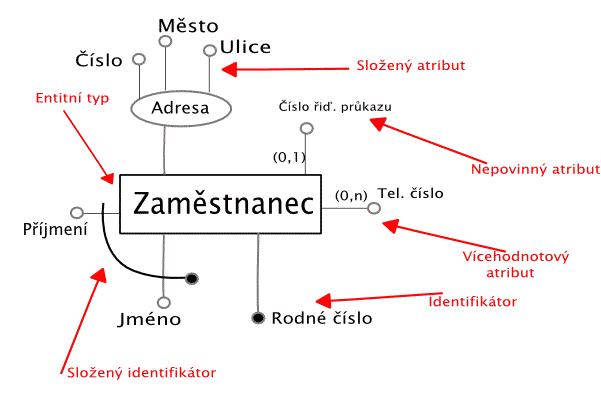
\includegraphics[width=14cm]{informatika/databazy/obrazky/er1.png}

(Entitní typ se všemožnými druhy atributů)
\end{center}
\end{obecne}

\begin{obecne}{Vztahový typ}
\emph{Vztahový typ} (v diagramu značený kosočtvercem) popisuje vztahy mezi jednotlivými entitami -- s těmi entitami, se kterými je v nějakém vztahu, je spojen čarou. Vztah může mít danou i \emph{kardinalitu} (kolik entit z každé strany do vztahu vstupuje), která může být typu $1:1$, $1:n$, $m:n$ a je značená vedle čáry spojující vztahový typ s entitou. Entity ve vztahu mohou mít navíc \emph{povinné či nepovinné členství} (vstupovat do něj vždy nebo jen někdy).

Vztahy mohou být buď binární nebo obecně $n$-ární, ale více než ternární vztahy se většinou neobjevují. Vztahy mohou být i rekurzivní, tj. do vztahů vstupují entity stejného typu. Instance vztahového typu je jednoznačně určena identifikátory instancí entit ve vztahu. Některé entitní typy mohou být spoluidentifikovány (nebo přímo identifikovány) vztahem -- pak se nazývají \emph{slabé entitní typy}.

\begin{center}
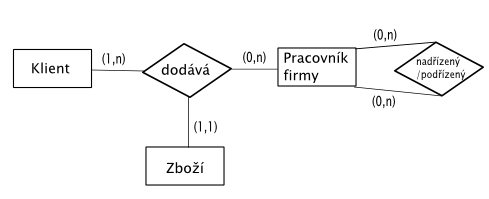
\includegraphics[width=12cm]{informatika/databazy/obrazky/er2.png}

(Vztahové typy)
\end{center}
Obrázek ukazuje ternární vztah s různými kardinalitami -- klientovi někdo dodává zboží jednou až $n$-krát, pracovník dodává nula až $n$-krát zboží (tj. jde o nepovinné členství ve vztahu, můžou existovat pracovníci, kteří nic nedodávají) a zboží je vždy někomu dodáváno právě jednou. Na zaměstnancích je zároveň ukázán rekurzivní binární vztah.


\begin{center}
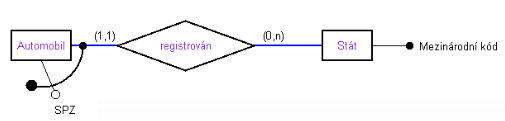
\includegraphics[width=10cm]{informatika/databazy/obrazky/er3.png}

(Slabý entitní typ. Zdroj: slidy Dr. T. Skopala k Databázovým systémům)
\end{center}
Tento obrázek ukazuje, jak vypadá slabý entitní typ -- automobil je identifikován svojí SPZ a zároveň státem, ve kterém je registrován.
\end{obecne}


\begin{obecne}{ISA hierarchie}
ISA hierarchie je rozšíření ER diagramů o \uv{dědičnost} entit -- tj. rozdělení entitních typů na subtypy (a přidání dalších vztahů nebo atributů pro subtypy). V ISA hierarchii se povoluje pouze jednonásobná dědičnost, navíc potomci nějakého entitního typu musí být jednoznačně identifikováni předkem (tj. všechny entity v hierarchii sdílí identifikátor).

\begin{center}
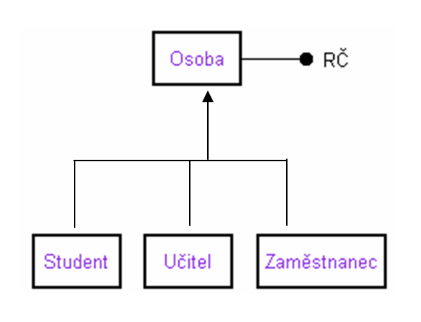
\includegraphics[width=6cm]{informatika/databazy/obrazky/er4.png}

(ISA hierarchie. Zdroj: slidy Dr. T. Skopala k Databázovým systémům)
\end{center}
\end{obecne}

\begin{obecne}{Úpravy ER diagramů}
V ER diagramu je možné provádět víceméně \uv{ekvivalentní} úpravy (výsledný diagram reprezentuje stejný koncept databáze), např. pro odstranění vztahů s kardinalitou $m:n$ (převod na dva vztahy kardinalitami $1:n$ a \emph{průnikový entitní typ}, který je vztahy určený, takže je slabý). Dalším důvodem úprav může být zbavení se ISA hierarchie. To se dá provést více způsoby, přičemž žádný z nich nefunguje úplně obecně:
\begin{pitemize}
    \item agregace atributů a vztahů potomka do předka a úprava kardinalit (převod na nepovinné atributy a nepovinné členství ve vztahu)
    \item odstranění předka a duplikace všech jeho atributů a vztahů v potomcích
    \item nahrazení ISA vztahu klasickým vztahem (z potomků vzniknou slabé entitní typy)
\end{pitemize}
Jiná úprava je odstranění vícehodnotového atributu -- převede se na vztah s kardinalitou $1:n$ a slabý entitní typ.
\end{obecne}

\begin{obecne}{Korektní ER schéma}
V \emph{korektním} ER schématu všechny entity a vztahy splňují:
\begin{pitemize}
    \item Žádný entitní typ nemá více než jednoho ISA předka.
    \item ISA vztahy netvoří orientovaný cyklus.
    \item Identifikační vztahy netvoří orientovaný cyklus.
    \item Potomek v ISA hierarchii není identifikačně závislý na žádném entitním typu (je již identifikován předkem).
    \item Jména entitních a vztahových typů jsou jednoznačná.
\end{pitemize}
\end{obecne}


TODO: Co je ksakru \uv{ metody návrhů IS}?
